
\thispagestyle{myheadings}
本章では,屋内位置推定ライブラリの要求仕様の検討およびその実装について述べる。
節3.1では要求仕様について詳述する.
節3.2では,軌跡の画像と関数を用いて,どのような補正を行っているかを示す.


\section{要求仕様}


\section{要求補正情報}
% TODO: 3.要求仕様ではなく要求補正情報の方がよさそう.要求仕様にするなら,柔軟性をもたせる設計にするとか書く必要がありそう.
% TODO: 3.要求仕様にしてこういう設計である必要があるという主張がいると思う.要求補正情報はおかしい
% TODO: これではまずい


PDRと他の情報を使ってライブラリを作成する上で,
どのような状況や環境が存在し補正に利用できるのかその具体的な例を考える必要がある.
例えば大学内や病院などのWi-FiのAPが多く設置されている場所では,
Wi-Fiの電波強度を利用した位置推定が有効である.
他の例として展示会場や大きなアトリウムなどの広い開放空間が考えられる.
このような場所ではWi-FiのAPの配置が難しく,
信号のカバレッジが不均一になりやすくWi-Fiを利用した位置推定は難しい.
このような場所の場合BLEビーコンを配置してその電波強度を利用した位置推定が有効である.
また2章で示したように\cite{pdr-wifi}\cite{pdr-ble}などのPDRと電波を利用した推定に関する研究は盛んに行われている.
このように電波を使った手法は多くの場所で有効であり,補正に利用可能な情報として重要度が高い.
そのため本ライブラリにおいても採用を行う.
他に補正に利用可能な情報としてフロアマップ情報がある.
フロアマップ情報は多くの場所で比較的入手が容易だと思われる.
そのため本ライブラリにおいても採用を行う.

磁気やカメラなどの情報は,磁気はデータが繊細であり電波と比べると補正に利用する難易度が高い,
カメラはプライバシーなどの問題があり本ライブラリの基礎段階においてこれらを採用しない.
また気圧センサは基礎段階として3次元空間を推定対象としないため採用しない.


\begin{figure}[ht]
	\centering
	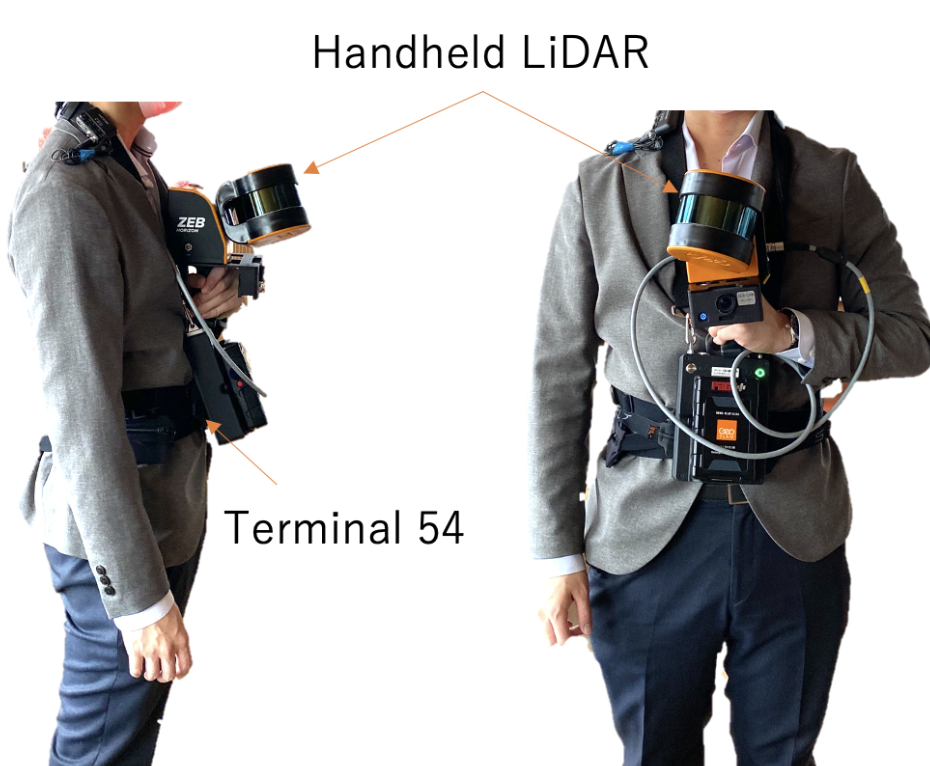
\includegraphics[width=\linewidth]{image/lidar.jpg}
	\caption{歩行者の装着器具}    \label{fig:step_detect}
\end{figure}






\section{ライブラリの実装}
3.21節ではxDR Challenge 2023環境における平面的な位置推定について述べる.
3.22節では気圧データを用いた3次元的な位置推定について述べる.

\subsection{xDR Challenge 2023環境における平面的な位置推定}


\subsection{基本的なPDR処理}

本ライブラリの基本的なPDR処理は,複数のクラスが協調して動作する設計となっている.
実装においては,コードの保守性と拡張性を重視し,Pythonの型ヒントやPandasライブラリを
効果的に活用している.特に,Pandasのデータフレーム構造を採用しており
大量のセンサデータに対する効率的な操作を実現している.また,時系列データのリサンプリングや
欠損値の補間,データの結合などの操作が容易に行えるため,センサデータの前処理や
解析に要する実装の複雑さを大幅に削減できる.
図\ref{fig:pdr-class}に示すように,PDREstimatorを中心として,StepEstimator,
OrientationEstimator,TrajectoryCalculatorの3つの主要なクラスが連携して
位置推定を行う.また,センサデータの管理はEnhancedSensorDataクラスが担当する.

\begin{figure}[H]
    \centering
    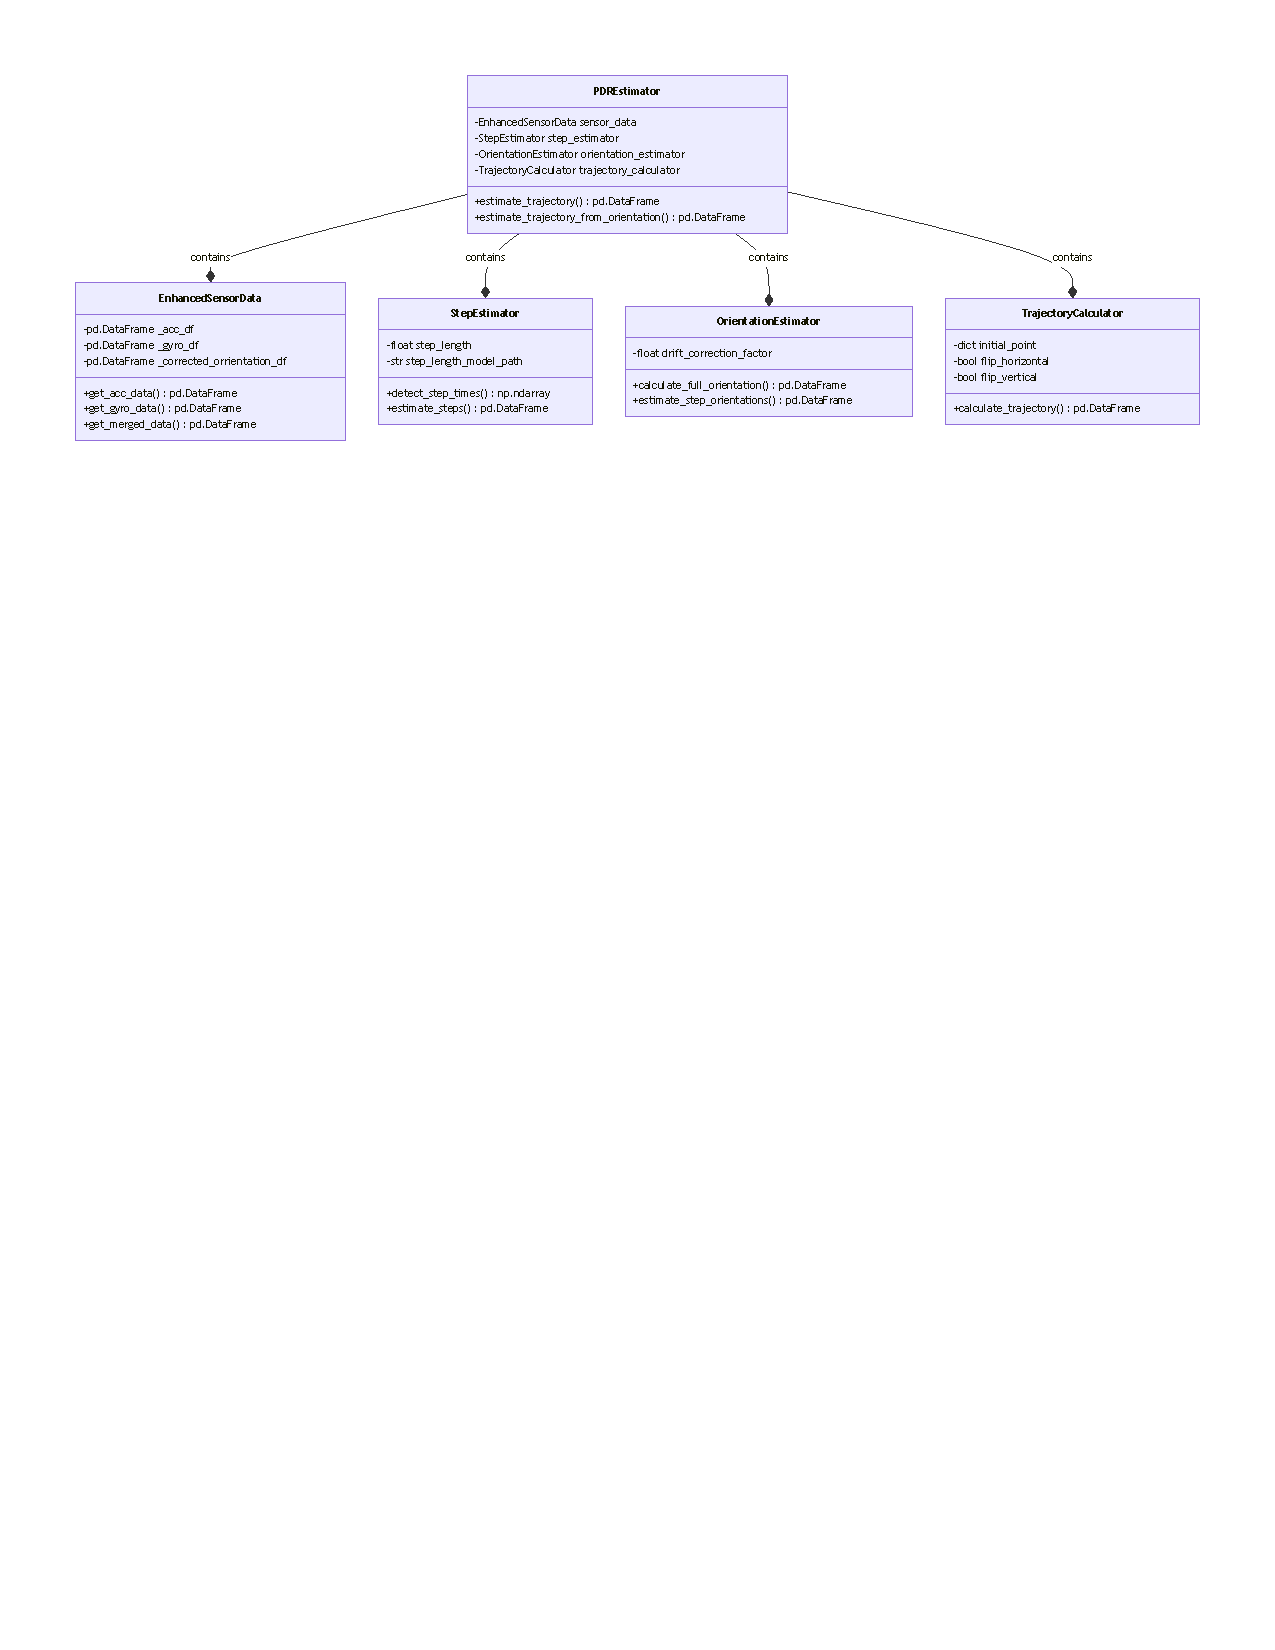
\includegraphics[width=\linewidth]{image/pdr-class-diagram.pdf}
    \caption{PDRの主要クラス構成}
    \label{fig:pdr-class}
\end{figure}

\subsubsection{システム構成}

本システムは,クラスベースの設計を行っている.各クラスの責任範囲を
明確に分離し,コードの理解性と保守性を向上させている.さらに,拡張可能な
インターフェース設計を採用しており,各クラスは明確なインターフェースを通じて相互に
連携するため,個々の実装の詳細を隠蔽しながら機能拡張が可能である.

各クラスの役割は以下の通りである:

\begin{description}
    \item[PDREstimator]\hfill 位置推定の中核となるクラスであり,他のコンポーネントを統括する.
    歩行検出,方向推定,軌跡計算の各処理を適切に連携させ,最終的な位置推定を行う.
    
    \item[EnhancedSensorData] 加速度,角速度などのセンサデータを管理する.データの前処理や
    同期処理を行い,他のコンポーネントに適切な形式でデータを提供する.
    
    \item[StepEstimator] 加速度データから歩行ステップを検出する.固定の歩幅を用いた
    シンプルな実装としており,拡張性を考慮した設計となっている.
    
    \item[OrientationEstimator] 角速度データから進行方向を推定する.ドリフト補正などの
    基本的な補正処理も行う.
    
    \item[TrajectoryCalculator] 検出された歩行ステップと推定された方向から,
    実際の移動軌跡を計算する.

\end{description}


\subsubsection{処理フロー}

PDRによる位置推定の処理フローを図\ref{fig:pdr-flow}に示す.本システムでは,センサデータの
入力から最終的な軌跡の出力まで,以下の段階を経て処理が行われる.

\begin{figure}[H]
    \centering
    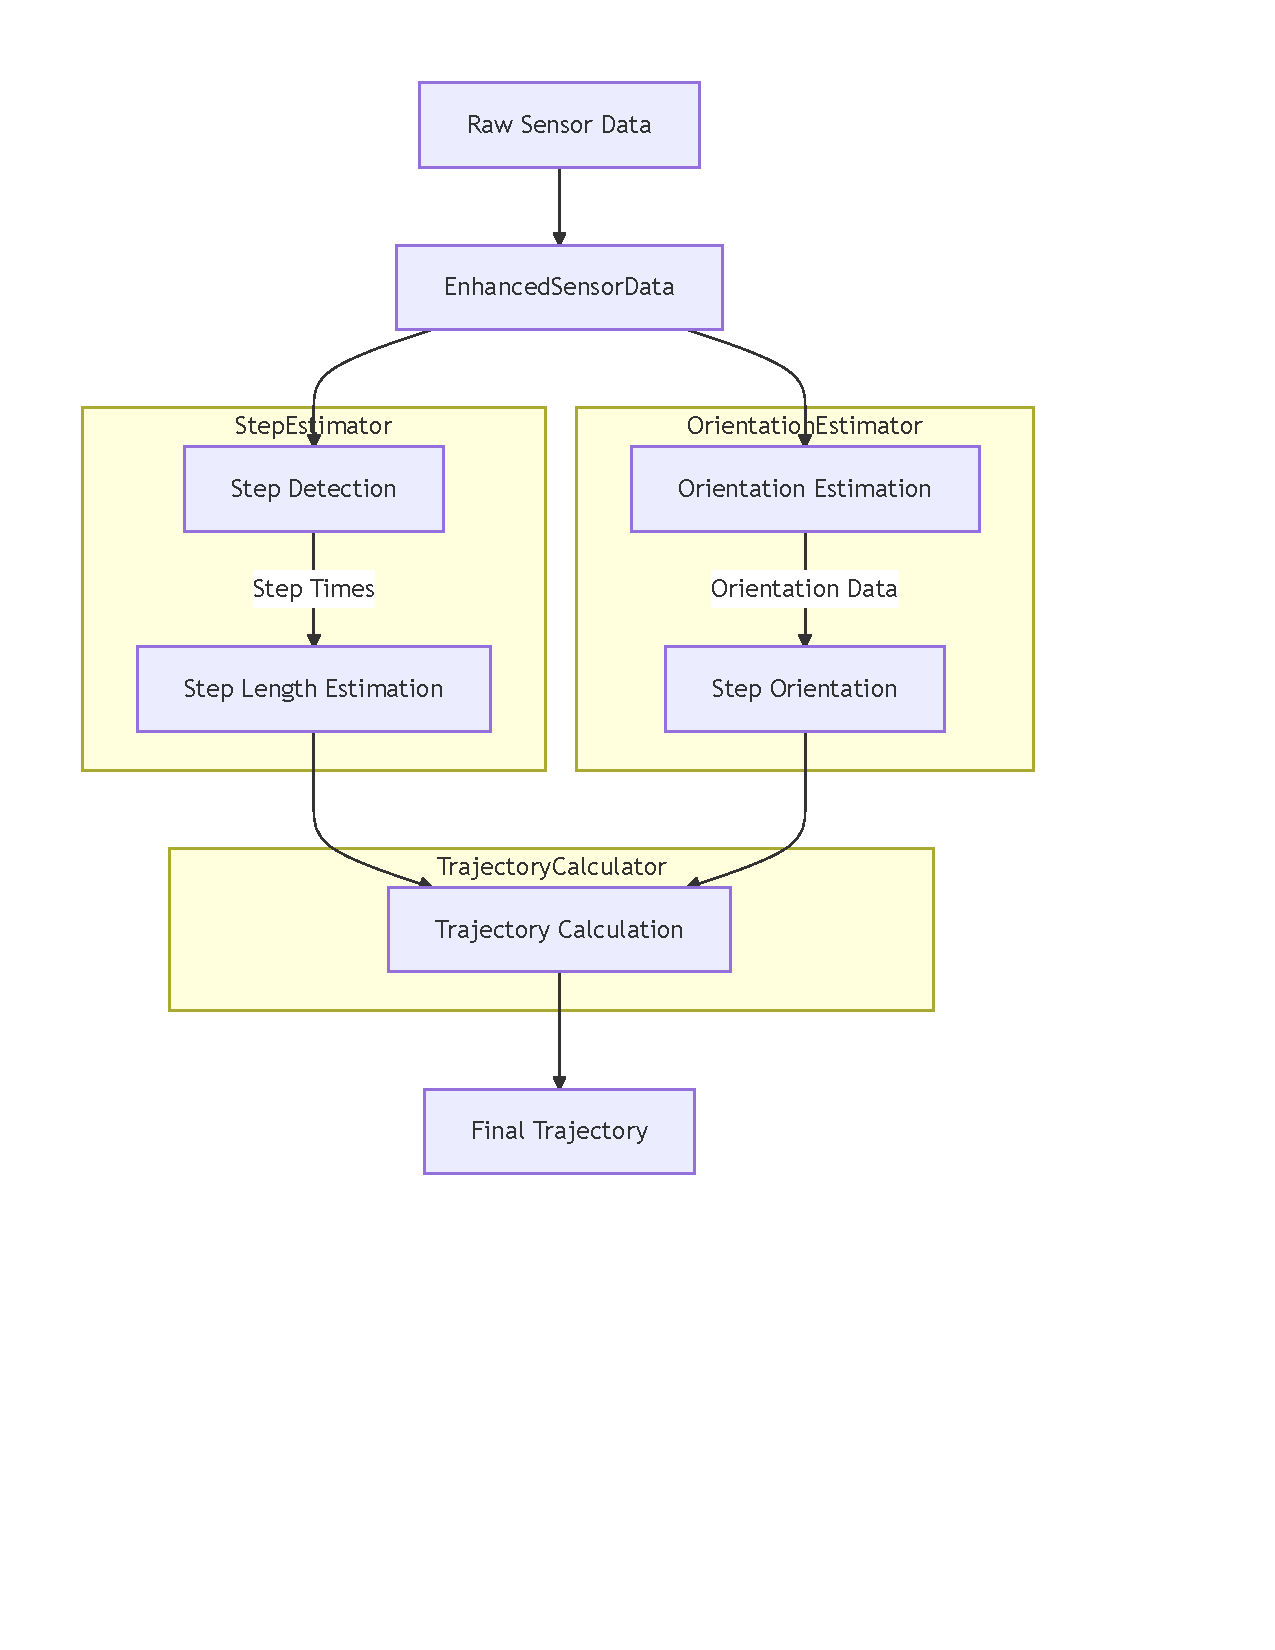
\includegraphics[width=\linewidth]{image/pdr-flow-diagram.pdf}
    \caption{PDRの処理フロー}
    \label{fig:pdr-flow}
\end{figure}

まずEnhancedSensorDataクラスにおいて,加速度センサと角速度センサから取得した生データの
前処理が行われる.前処理では,データの同期やノイズ除去などの基本的な処理に加え,
後続の処理で扱いやすい形式への変換が行われる.具体的には加速度データと角速度データの
サンプリング周波数の違いを考慮し,時系列データの補間処理を行い,両者のタイムスタンプを
一致させる.これにより後続の処理での時系列データの扱いが容易になる.


次に,StepEstimatorクラスにおいて歩行ステップの検出と歩幅の推定が行われる.
図\ref{fig:step_detect}に示すように,歩行ステップの検出では3軸加速度の
ノルムを計算し,その値が閾値を超えた時点を歩行ステップとして検出する.
具体的には,まず加速度のノルムに対して平滑化処理を適用し,
ノイズの影響を軽減する.
この際,単純な固定閾値ではなく,適応的な閾値処理を採用している.システムは
加速度信号の特性を継続的に監視し,平均値と標準偏差を用いて動的に閾値を
調整する.図\ref{fig:step_detect}の赤い破線で示されているように,
閾値は加速度の平均値に標準偏差の一定倍を加えた値として計算される.
この適応的な閾値の採用により,歩行速度の変化や個人差による加速度パターンの
違いに柔軟に対応できる.また信号の品質が時間とともに変化する
場合でも,安定した歩行検出が可能となる.図中の赤い点が,この適応的な
閾値処理によって検出された歩行ステップを示している.

同時にOrientationEstimatorクラスでは角速度データを用いた方向推定を行う.
図\ref{fig:step_timing}に示すように,角速度の積分により進行方向を算出する.
図中の青線は推定された進行方向の変化を,赤点は各歩行ステップでの方向を示している.
ただし積分処理には誤差の蓄積(ドリフト)という問題が存在する.
そのため本実装ではあらかじめドリフトの値が判明している場合,線形ドリフト補正を適用できるようにしている.
具体的には時間経過に比例する形でドリフト量を推定し,その影響を除去する処理を行う.

最後にTrajectoryCalculatorクラスにおいて,検出された歩行ステップと推定された
方向の情報を組み合わせて実際の移動軌跡を計算する.この過程では以下の式を用いて座標を逐次的に更新する:

\begin{equation}
x_{n+1} = x_n + L \cos(\theta_n)
\end{equation}
\begin{equation}
y_{n+1} = y_n + L \sin(\theta_n)
\end{equation}

ここで,$(x_n, y_n)$は$n$番目のステップでの位置,$L$は歩幅,$\theta_n$はその時点での
推定進行方向を表す.また,初期位置が与えられている場合は,その値を$(x_0, y_0)$として
使用する.さらに,座標系の定義に応じて,必要な座標変換(x軸やy軸の反転など)も
この段階で適用される.
% TODO: ここに中間報告で使用した計算が積み重なっていくのがわかる図があるといいかも

このように,各クラスが明確な役割分担の下で連携し,PDRによる位置推定を
実現している.また,この設計により,各処理段階での改良や機能追加が容易となっている.
例えば,より高度な歩行検出アルゴリズムの導入や,新たな方向推定手法の実装などが,
他のコンポーネントに影響を与えず可能である.


\begin{figure}[H]
	\centering
	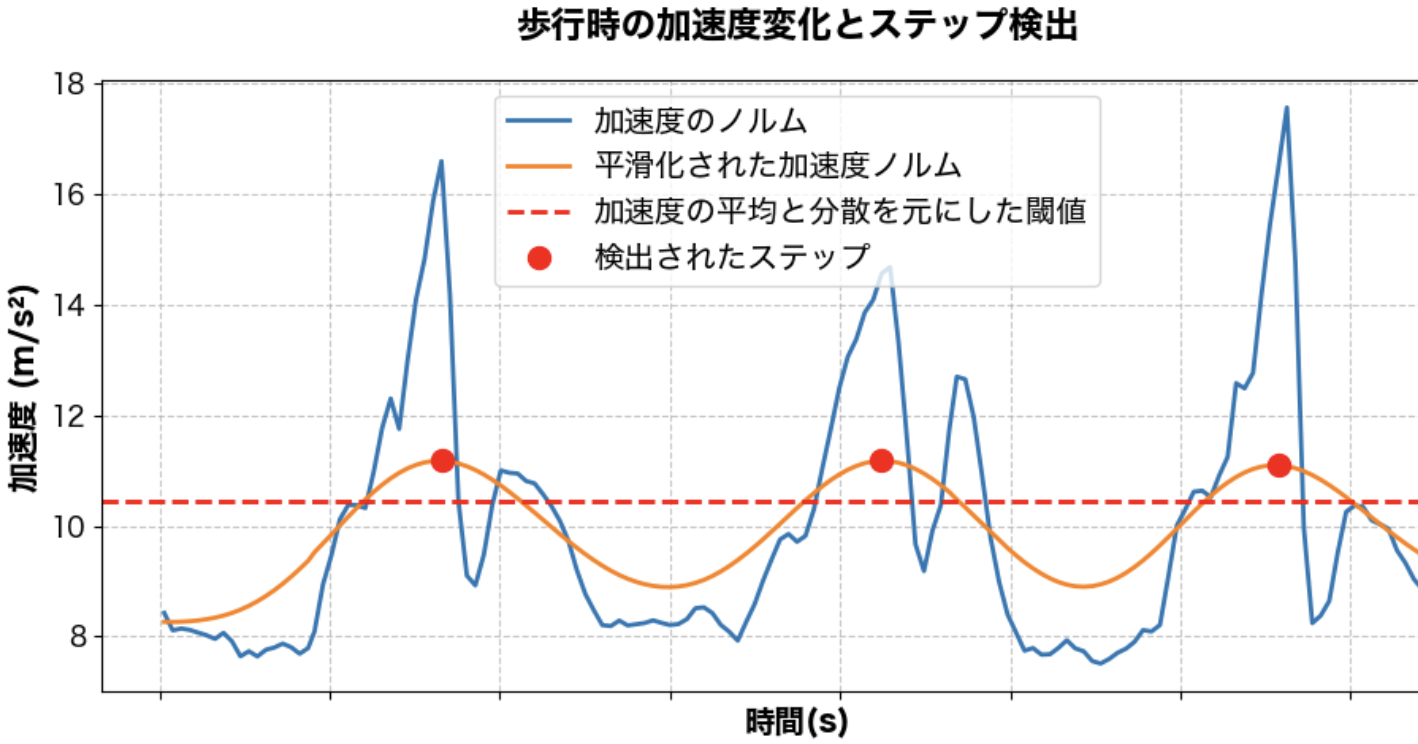
\includegraphics[width=\linewidth]{image/step_detect.jpg}
	\caption{加速度を利用したステップ検出}    \label{fig:step_detect}
\end{figure}


\begin{figure}[H]
	\centering
	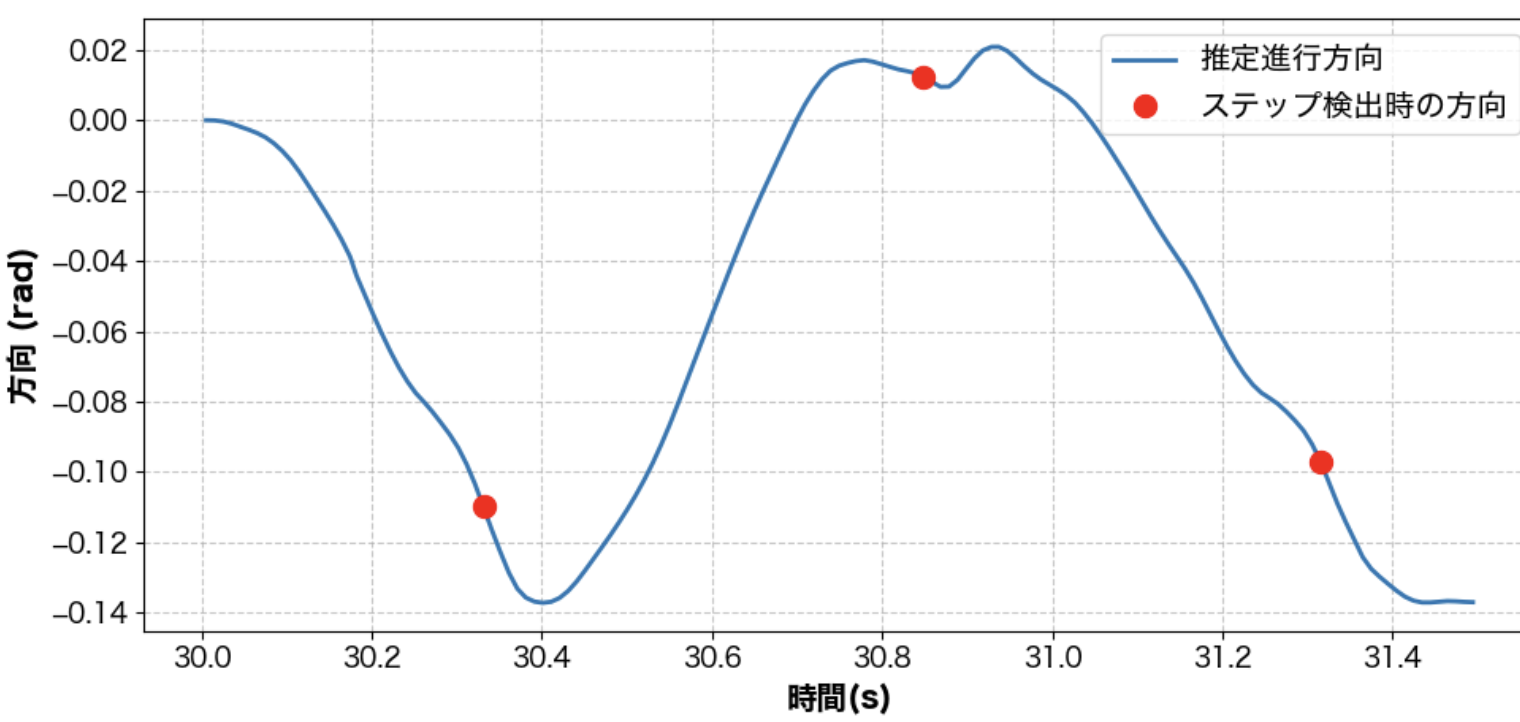
\includegraphics[width=\linewidth]{image/step_timing_angle.jpg}
	\caption{推定進行方向の変化}    \label{fig:step_timing}
\end{figure}


xDR Challenge 2023で与えられたトレーニングセンサーデータに対して処理を行った例を示す.
図\ref{fig:pdr}はPDREstimatorによる位置推定を行った結果である.
この図は2次元座標上に推定軌跡を表しており,軌跡の色は経過時間を表している.
紫色から赤色への変化が時間の経過を示している.
TrajectoryCalculatorに正解初期座標を与えた結果が図\ref{fig:pdr-move}である.
この図から分かるように,予め正解座標が判明している場合はPDRによる軌跡の初期位置を
適切に補正することができる.比較のため,LiDARで取得した座標を基に出力された
軌跡を図\ref{fig:gt-trajectory}に示す.これを本論では正解軌跡として扱う.
図\ref{fig:pdr-move}と図\ref*{fig:gt-trajectory}を比較すると,初期位置を補正した
PDRによる軌跡であっても,正解軌跡と比べて大きく異なっていることが分かる.
これはPDR特有の問題として,以下の2つの課題が存在するためである:

\begin{itemize}
    \item 相対的な移動の累積による軌跡の歪み
    \item 実世界の座標系における正確な位置の特定
\end{itemize}


続く3.2節では,これらの問題に対して軌跡補正クラスを用いたアプローチを示し,
PDRの軌跡を正解軌跡に近づけていく手法について詳しく説明する.


\begin{figure}[H]
    \centering
    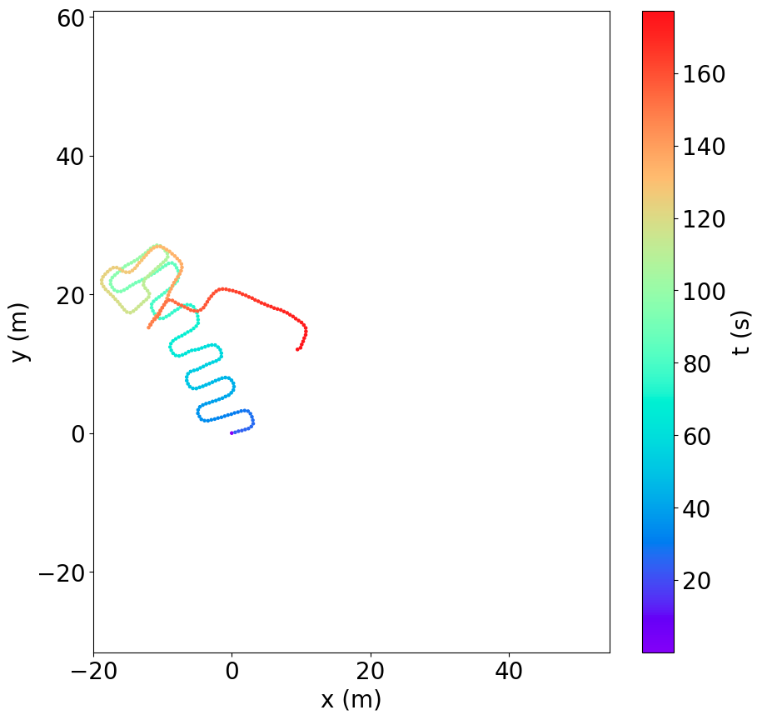
\includegraphics[width=\linewidth]{image/pdr.jpg}
    \caption{基本PDRの軌跡}    \label{fig:pdr}
\end{figure}


\begin{figure}[H]
    \centering
    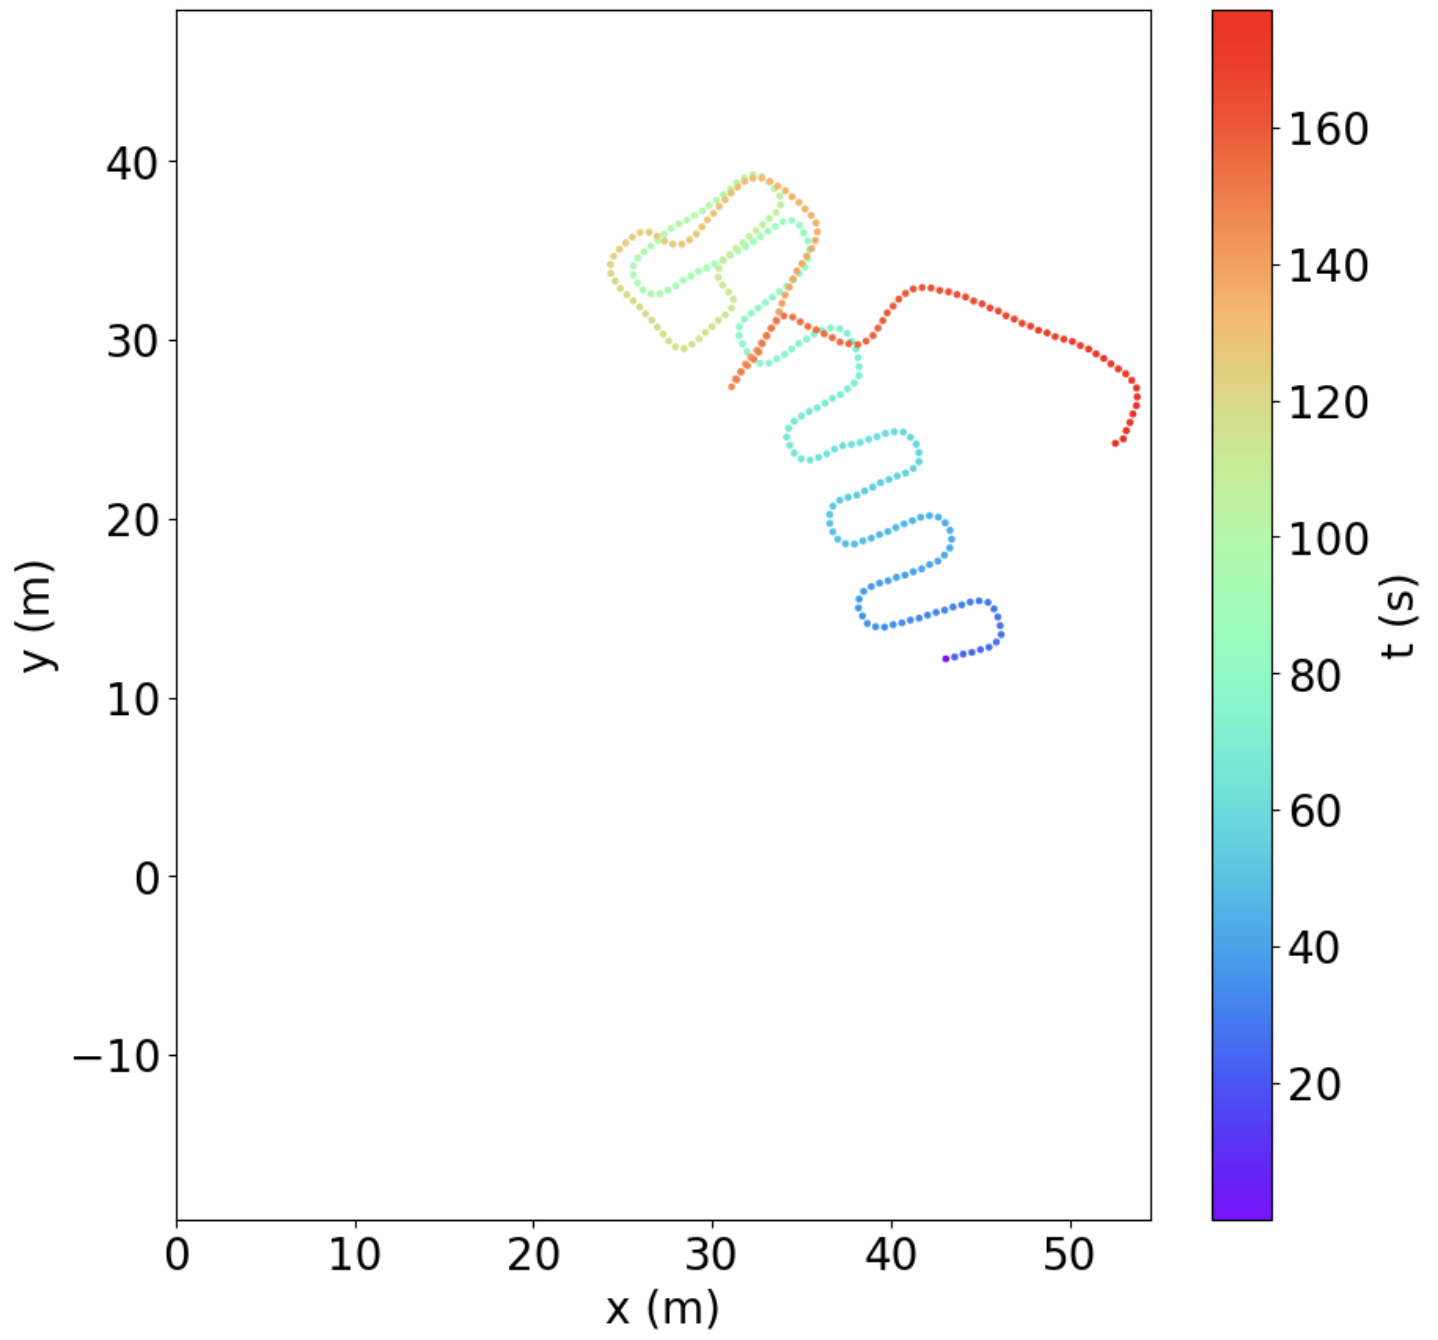
\includegraphics[width=\linewidth]{image/pdr-move.jpg}
    \caption{正解初期座標が存在}    \label{fig:pdr-move}
\end{figure}


\begin{figure}[H]
    \centering
    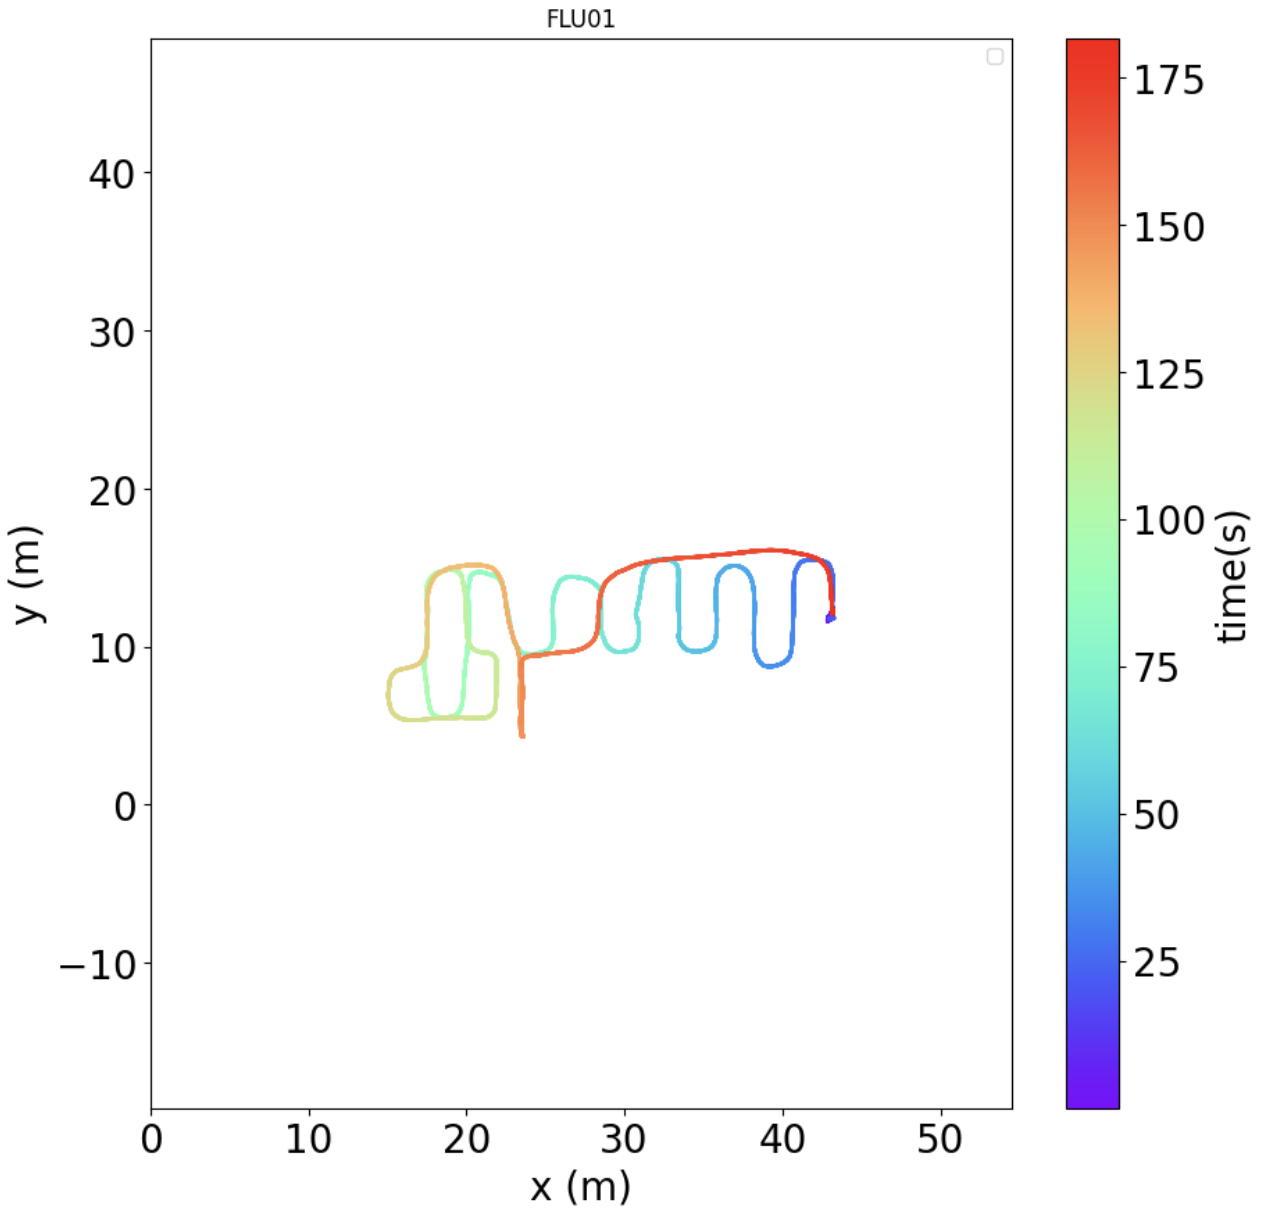
\includegraphics[width=\linewidth]{image/gt2.jpg}
    \caption{正解軌跡}    \label{fig:gt-trajectory}
\end{figure}















図\ref{fig:pdr-move}の軌跡にはPDR特有のドリフト現象が見られる.
PDRでは角速度から進行方向を求めてその方向を元に歩行軌跡を描く.
そのため角速度センサーにわずかでも誤差が含まれると,時間経過とともにその誤差が大きくなり軌跡の形状が本来の軌跡から外れる.
この問題を解決するには角速度データに含まれる累積誤差を取り除く必要がある.


\begin{lstlisting}[caption={ドリフト除去}, label=lst:remove-drift,float =h]
def remove_drift_in_angle_df(
    acc_df: pd.DataFrame,
    angle_df: pd.DataFrame,
    ground_truth_point_df: pd.DataFrame,
) -> tuple[pd.DataFrame, pd.DataFrame]:
\end{lstlisting}

ドリフトを取り除く関数をListing\ref{lst:remove-drift}に示す.
引数として加速度DF,角速度DF,正解座標DFを受け取る.
戻り値は角度DFと座標DFを返す.
ドリフト補正のプロセスは,ドリフトの値を動的に計算し,それを各時刻の角度データから差し引く.
このドリフト補正プロセスは,式(1)で表される.
$\theta'(t)$は時間$t$における補正後の角度,$\theta(t)$は補正前の角度,
$\mathrm{d}$はドリフトの大きさを意味する.
この式は時間経過に伴うドリフトの累積効果を補正するために使用される.


\vspace{5mm} % 5mmの空白を追加。必要に応じて値を調整してください。
\begin{equation}
	\theta'(t) = \theta(t) - (\mathrm{d} \times (t))
\end{equation}

\vspace{5mm} % 5mmの空白を追加。必要に応じて値を調整してください。

補正の効果を評価し適切なドリフトを見つけるために,ユークリッド距離を用いて,2つの正解座標の差異を計算する.
式(2)は,正解座標$(x_{\mathrm{n}}, y_{\mathrm{n}})$と正解座標$(x_{\mathrm{n+1}}
	y_{\mathrm{n+1}})$との間のユークリッド距離$\mathrm{E}$を示している.
この式に基づきドリフト値に対してグリッドサーチを行い距離が最小になるドリフト値を探す.
最小のドリフト値を角度DFから引きそれに基づいた座標DFと角度DFを返す.
図\ref{fig:pdr-remove-drift}に示すように,ドリフト補正後の軌跡は,元の軌跡と比較して正解軌跡の形状に近づいている.
このアルゴリズムでは正解座標$(x_{\mathrm{n}}, y_{\mathrm{n}})$と
正解座標$(x_{\mathrm{n+1}}, y_{\mathrm{n+1}})$の距離が近い時に特に有効である.
この処理は$(x_{\mathrm{n+2}}, y_{\mathrm{n+2}})$など2つ以上の座標が存在する場合も同様に適用できる.

\vspace{5mm} % 5mmの空白を追加。必要に応じて値を調整してください。
\begin{equation}
	\mathrm{E} = \sqrt{(x_{\mathrm{n+1}} - x_{\mathrm{n}})^2 + (y_{\mathrm{n+1}} - y_{\mathrm{n}})^2}
\end{equation}
\vspace{5mm} % 5mmの空白を追加。必要に応じて値を調整してください。

\begin{figure}[h]
	\centering
	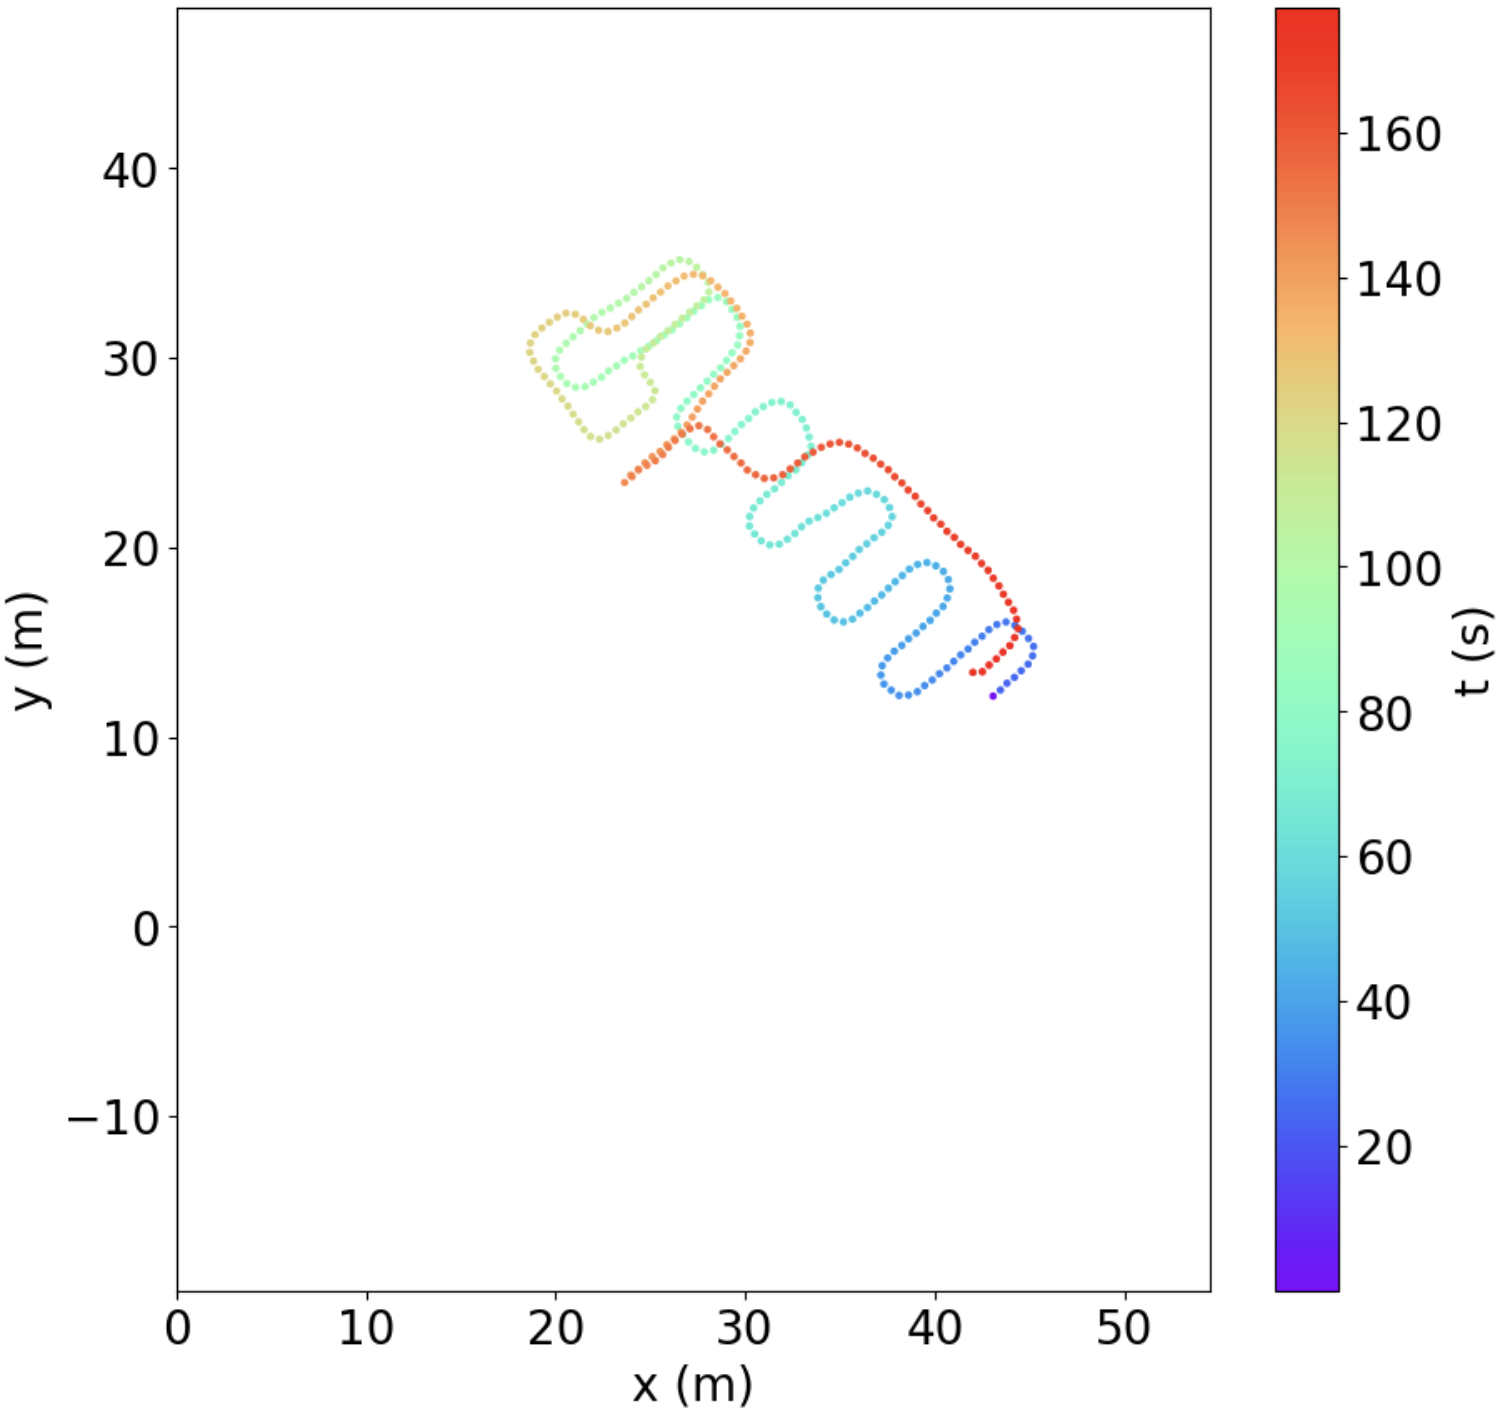
\includegraphics[width=\linewidth]{image/pdr-remove-drift-two.jpg}
	\caption{ドリフト補正後の軌跡}    \label{fig:pdr-remove-drift}
\end{figure}



\subsubsection{フロアマップを用いた初期進行方向の補正}

図\ref{fig:pdr-remove-drift}の軌跡には,初期進行方向の誤差という重要な
問題が残されている.初期進行方向が誤っていると,その後の全ての推定位置が
実際の移動経路から大きく逸れることになる.この問題に対処するため,本ライブラリ
ではMapMatcherクラスを提供している.

MapMatcherクラスは,フロアマップの構造的特徴を利用して最適な初期進行方向を
推定する.この手法は,
多くの屋内環境において壁や通路が直交する形で構成されている
という特徴を活用している.
図\ref{fig:floor-map}に実際のフロアマップを示す.
このマップの灰色の部分が歩行可能領域であり,白色の部分が歩行不可能領域である.
図\ref{fig:floor-map}に示すような実際のフロアマップでは,
歩行可能な経路の多くが建物の主軸に沿って配置されている.

\begin{figure}[H]
	\centering
	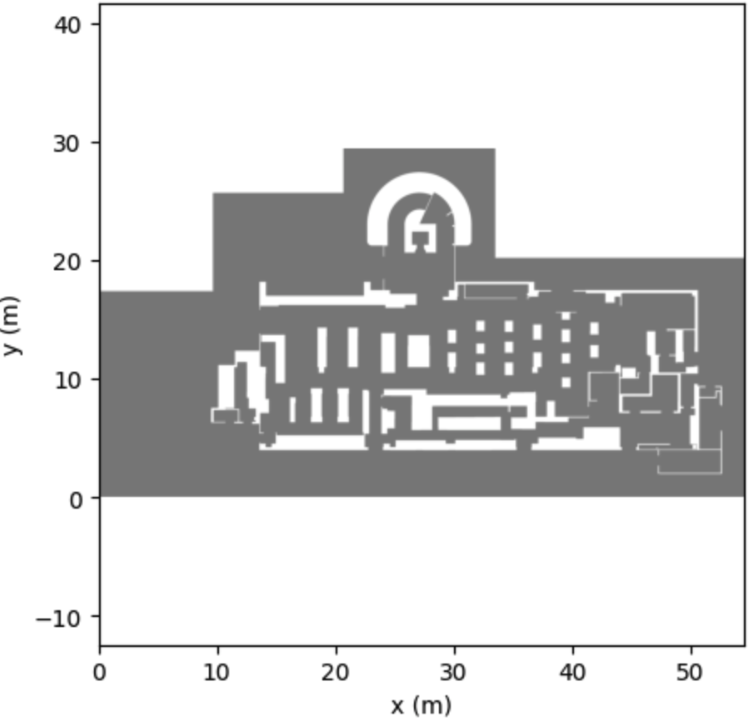
\includegraphics[width=\linewidth]{image/floor-map.jpg}
  \caption{フロアマップ情報} \label{fig:floor-map}
\end{figure}

初期進行方向の推定は,以下の2段階のプロセスで行われる:

第一段階では,軌跡のx軸,y軸に対して平行な成分の割合を最大化する角度を探索する.
具体的には,進行方向の角度が垂直方向(90度または270度)に対して±0.1ラジアン以内,
または水平方向(0度または180度)に対して±0.1ラジアン以内の歩行ステップを平行な
成分としてカウントする.この閾値は,人間の通常の歩行では廊下や通路に対して
完全に平行でなくとも,概ねその方向に沿って歩く傾向があることを考慮して設定されている.

図\ref{fig:parallel}は,異なる回転角度での軌跡における平行成分の分布を比較したものである.
赤い点はx軸またはy軸に対して平行な成分を,青い点はそれ以外の成分を示している.
左側の例では平行な成分の割合が少なく,軌跡が建物の主軸に対して斜めに配置されている.
一方,右側の例では平行な成分の割合が多く,軌跡が建物の構造とよく整合している.
このように,平行成分の割合を分析することで,建物の主軸に整合する可能性の高い
角度を特定することができる.ただし,この情報だけでは4つの候補角度(0度,90度,180度,
270度)のうち,どの角度が最適であるかを一意に決定することはできない.

\begin{figure}[H]
	\centering
	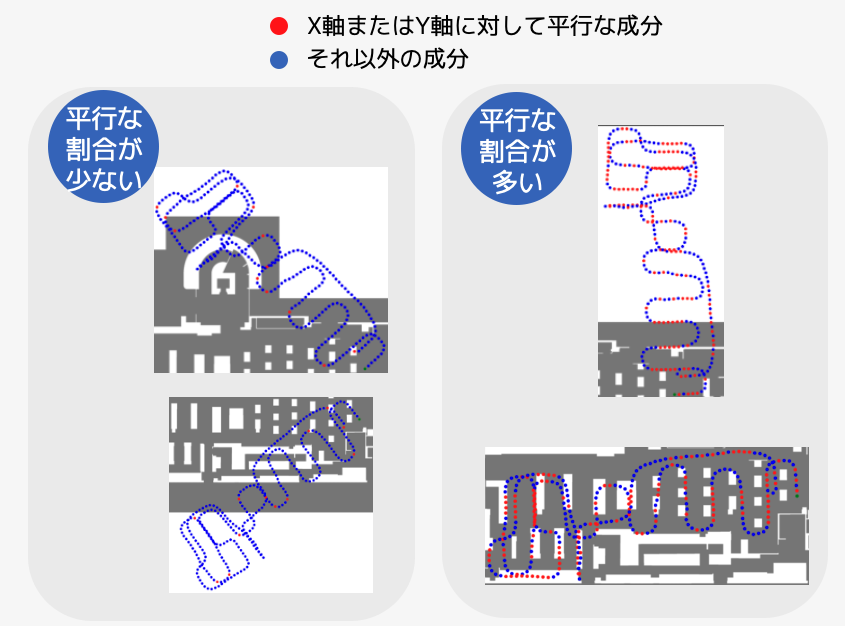
\includegraphics[width=\linewidth]{image/parallel.jpg}
	\caption{x軸とy軸に関して平行な成分の割合}    \label{fig:parallel}
\end{figure}

第二段階では,フロアマップ上の歩行可能領域の情報を活用する.
具体的には,各候補角度で軌跡を回転させ,その軌跡上の点がフロアマップ上で歩行可能な
領域に含まれる割合を計算する.MapMatcherは以下のようなコードで
使用される:

% TODO:3.ここに第2段階の図を載せる(後で可視化した図を作成する)

\begin{lstlisting}
# MapMatcherの初期化
map_matcher = MapMatcher(
    config={},             # 設定パラメータ
    pdr_estimator=estimator,  # PDREstimatorインスタンス
    floor_map=floor_map    # フロアマップ情報
)

# 初期進行方向の補正
corrected_trajectory = map_matcher.correct_initial_direction()
\end{lstlisting}

図\ref{fig:pdr-rotate}は,この補正処理を適用した結果を示している.
補正後の軌跡は建物の構造に整合し,正解軌跡により近い形状となっている.
この手法は,特に廊下や部屋が格子状に配置された一般的なオフィスビルなどの
環境で効果的である.

\begin{figure}[H]
	\centering
	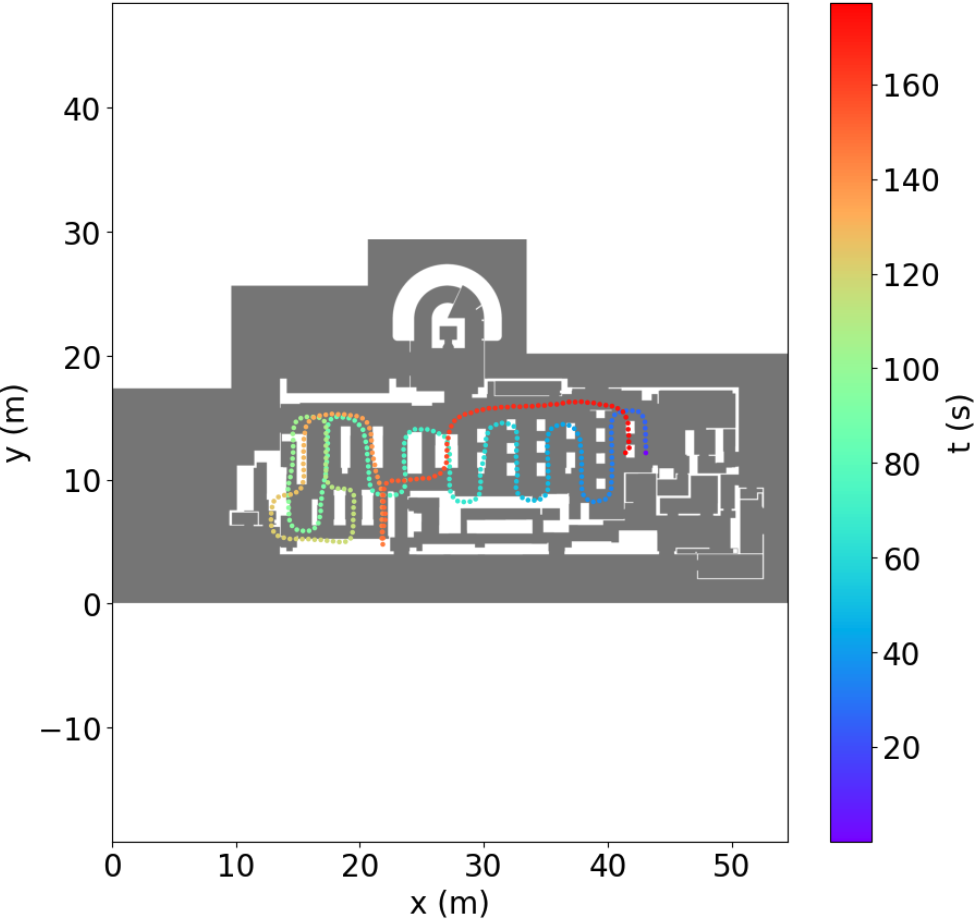
\includegraphics[width=\linewidth]{image/pdr-rotate.jpg}
	\caption{初期進行方向の補正後の軌跡}    \label{fig:pdr-rotate}
\end{figure}




フロアマップ情報を用いた初期進行方向補正ではマップの
存在可能な点の分布によっては正しく機能しない場合があり,
別の方法としてBLEビーコンの基地局の位置情報を用いた
初期進行方向補正を行う関数をListing\ref{lst:rotate-trajectory-using-ble}に示す.
この関数では加速度DF,角度DF,BLEビーコンの受信電波DF, BLEビーコンの基地局DFを受け取る.
BLEビーコンの受信電波DFとBLEビーコンの基地局DFのカラム名とデータ型を表6,表7に示す.
戻り値は角度DFと座標DFを返す.
フロアマップ上に存在する全てのBLEビーコンの基地局の位置情報を図\ref{fig:ble-beacon-position}に示す.
一定の強いRSSIの電波を受信した際の時間情報を基に時間的に近い推定軌跡の座標を取得する.
図\ref{fig:ble-merge}に示した図は時間的に近い推定軌跡の座標を時間経過に応じた色で表しており
青色の座標が配置されたBLEビーコンの座標を表している.
推定した軌跡の受信したBLEビーコンの基地局の座標との距離を計算する.
この総和が最小となるような回転角度をグリッドサーチで探し最適な角度に補正を行う.

\begin{lstlisting}[caption={BLEビーコンの基地局の位置情報を\\使用した初期進行方向補正}, label=lst:rotate-trajectory-using-ble]
def rotate_trajectory_to_optimal
		_alignment_using_ble(
    acc_df: pd.DataFrame,
    angle_df: pd.DataFrame,
    ble_scans_df: pd.DataFrame,
    ble_position_df: pd.DataFrame,
    ground_truth_first_point: dict[Axis2D, float]
) -> tuple[pd.DataFrame, pd.DataFrame]:
\end{lstlisting}


\begin{figure}[ht]
	\centering
	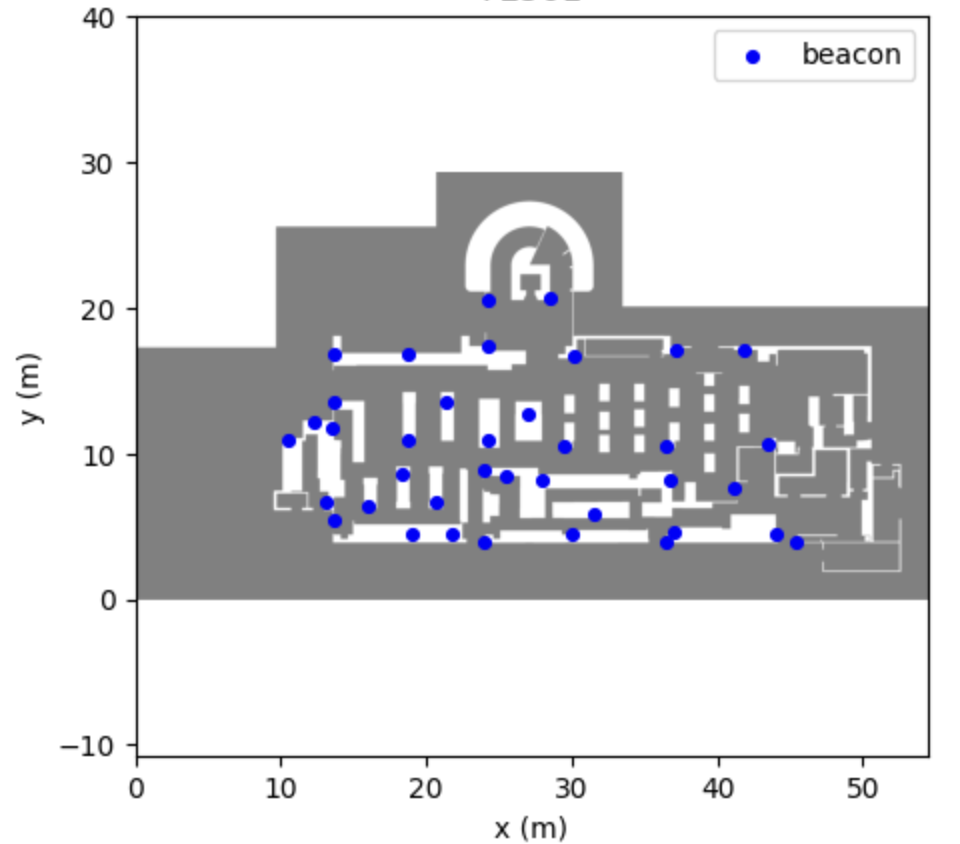
\includegraphics[width=\linewidth]{image/ble-beacon-position.jpg}
	\caption{BLEビーコンの基地局の位置情報}    \label{fig:ble-beacon-position}
\end{figure}

\begin{figure}[ht]
	\centering
	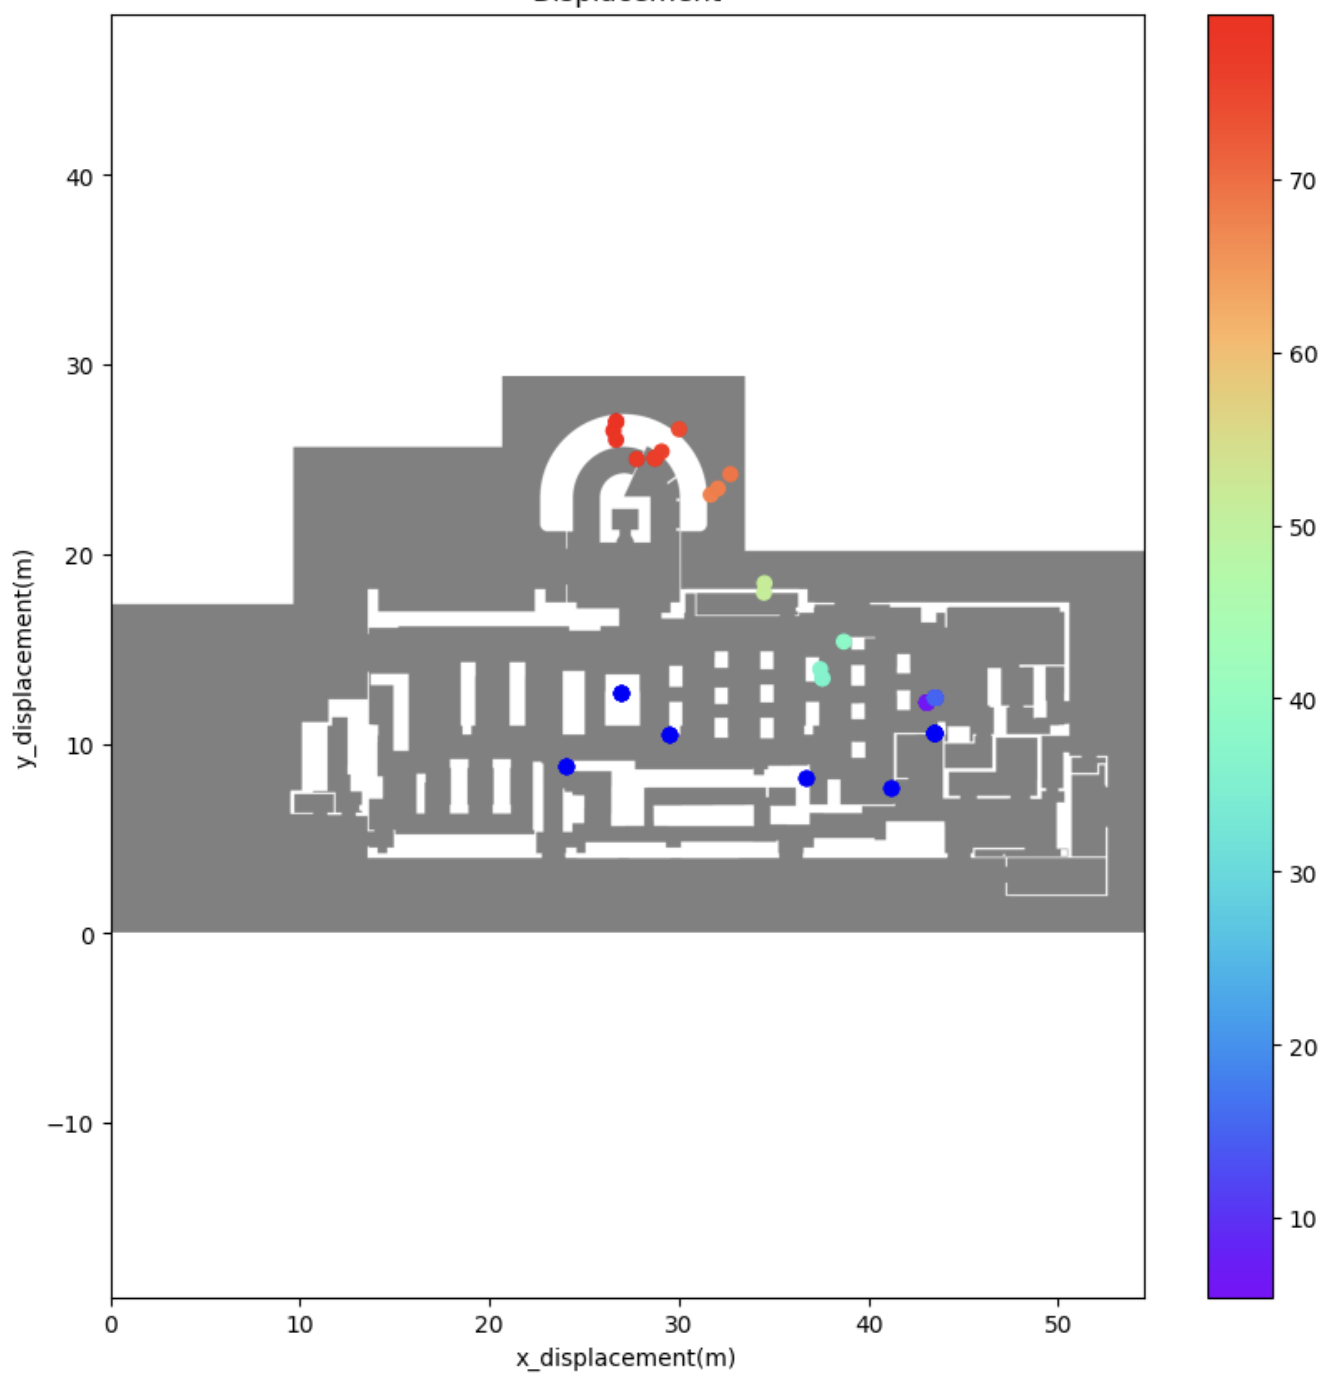
\includegraphics[width=\linewidth]{image/ble-merge.jpg}
	\caption{強いビーコン電波を受信した際の\\時間的に近い軌跡の座標}    \label{fig:ble-merge}
\end{figure}

\begin{table}[ht]
  \caption{BLEビーコンの受信電波 DF}
	\centering
	\begin{tabular}{lll}
		\toprule
		カラム名      & 単位    & データ型  \\
		\midrule
		ts        & s (秒) & float \\
		bdaddress & なし    & str   \\
		rssi      & dBm   & int   \\
		\bottomrule
	\end{tabular}
\end{table}

\begin{table}[ht]
	\caption{BLEビーコン基地局 DF}
	\centering
	\begin{tabular}{lll}
		\toprule
		カラム名        & 単位 & データ型  \\
		\midrule
		bdaddress   & なし & str   \\
		x           & m  & float \\
		y           & m  & float \\
		floor\_name & なし & str   \\
		\bottomrule
	\end{tabular}
\end{table}



\subsection{BLE FPを用いた初期進行方向の補正}

BLEビーコンの基地局の位置情報を基に初期進行方向の補正を行ったが
常にそれが利用可能であるとは限らない.
電波を使った手法としてWi-Fiを使った手法もあるがこの場合も同様であり
基地局の位置情報の把握にはコストがかかる場合がある.
基地局の位置情報を用いない代替手法としてFPを用いた手法がある.
この手法は,事前に特定の場所で受信したBLEビーコンのIDと
電波強度のデータを蓄積しておく必要があり,そのデータを基に
受信したIDとRSSIの値から位置を推定する.
この手法を用いて初期進行方向を補正する関数を
Listing\ref{lst:rotate-trajectory-using-ble-fingerprint}に示す.
この関数は引数に加速度DF,角度データDF,BLEビーコンの受信電波DF,
BLEビーコンのFPDF,フロア名を受け取る.
戻り値は角度DFと座標DFを返す.
受信電波情報とFPを基に推定した座標を示したのが図\ref{fig:fingerprint-location}である.
図の青色の点が受信したBLEビーコンの基地局座標であり,
赤色の点がこの基地局から受信した電波とFPを基に位置を推定した座標である.
理解しやすいように図中では受信したIDが1つのみを表示しているが,
実際は複数の強い電波を受信した点が存在する.
また説明のために基地局情報を示しているが今回の使用ケースでは
この座標は判明していないのが前提である.
この関数の内部処理では上記で示した受信電波情報とFPを基に推定した座標と
推定軌跡の座標との距離の総和を用いて,
その和が最小となる角度を探す.
BLEビーコンの基地局情報を基に初期進行方向を回転させた際と,ほぼ同様の結果が得られた.


\begin{table}[ht]
  \caption{BLEビーコンのFP DF}
	\centering
	\begin{tabular}{lll}
		\toprule
		カラム名        & 単位      & データ型  \\
		\midrule
		ts          & s (秒)   & float \\
		x           & m(メートル) & float \\
		y           & m(メートル) & float \\
		z           & m(メートル) & float \\
		bdaddress   & なし      & str   \\
		rssi        & dBm     & int   \\
		floor\_name & なし      & str   \\
		\bottomrule
	\end{tabular}
	\label{table:ble-beacon-fingerprint-df}
\end{table}


\begin{figure}[ht]
	\centering
	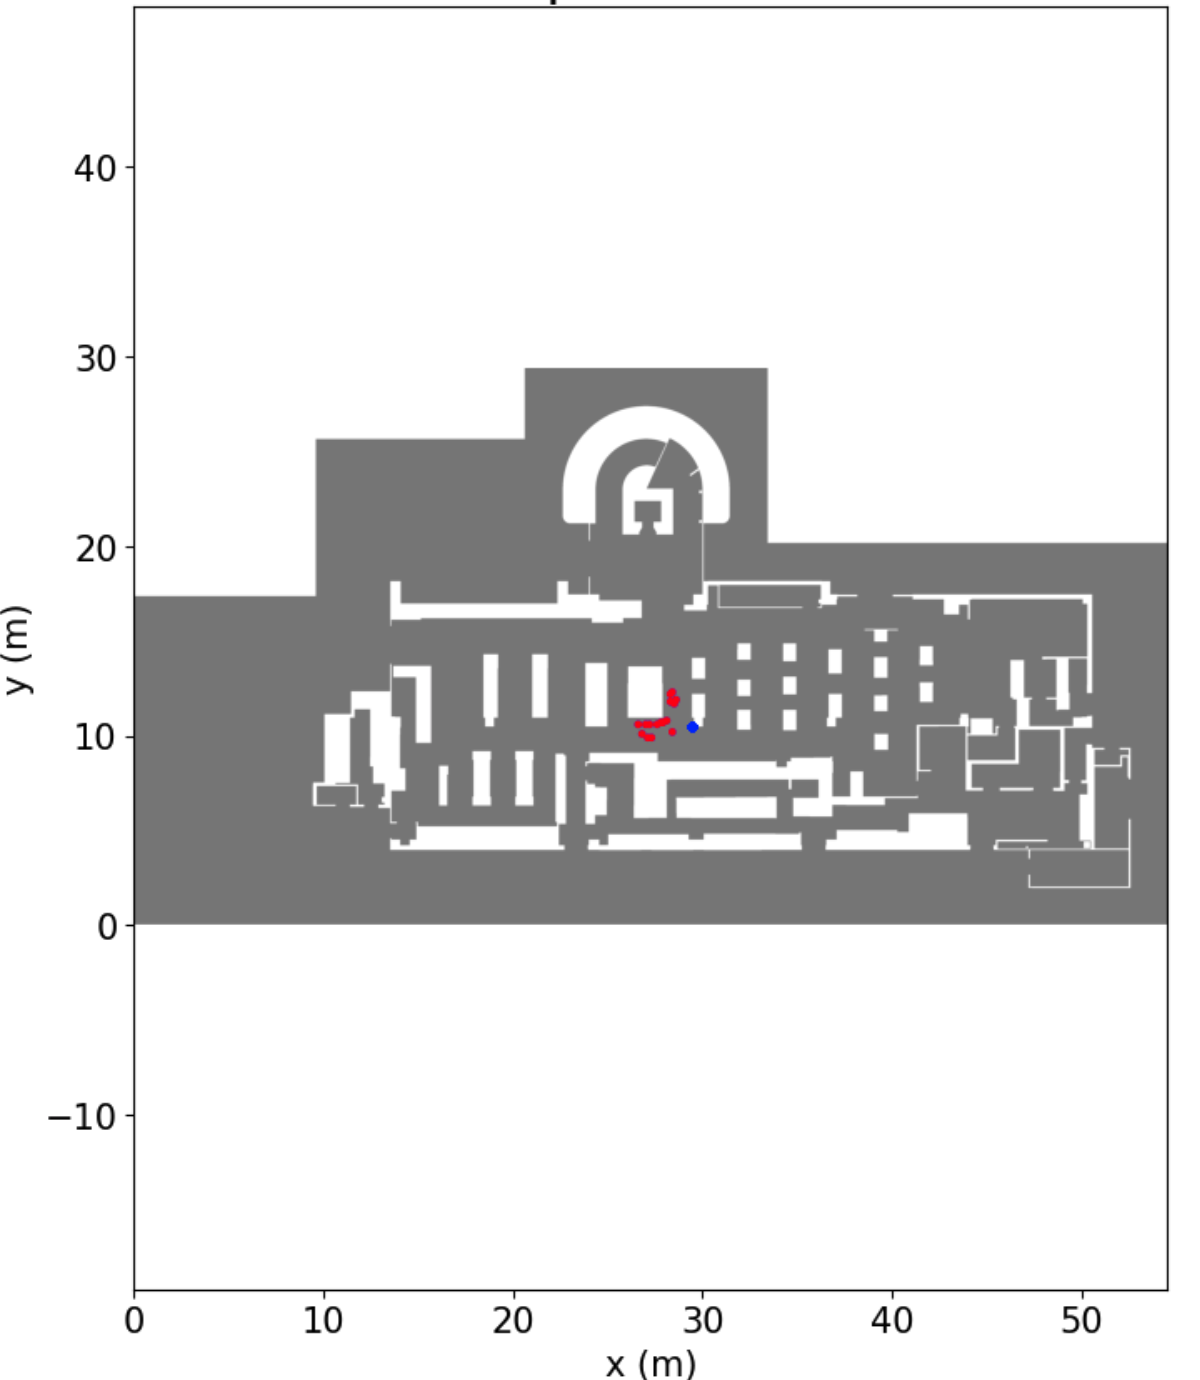
\includegraphics[width=\linewidth]{image/fingerprint-location.jpg}
	\caption{FPに基づく位置の推定}    \label{fig:fingerprint-location}
\end{figure}


\begin{figure}[ht]
	\centering
	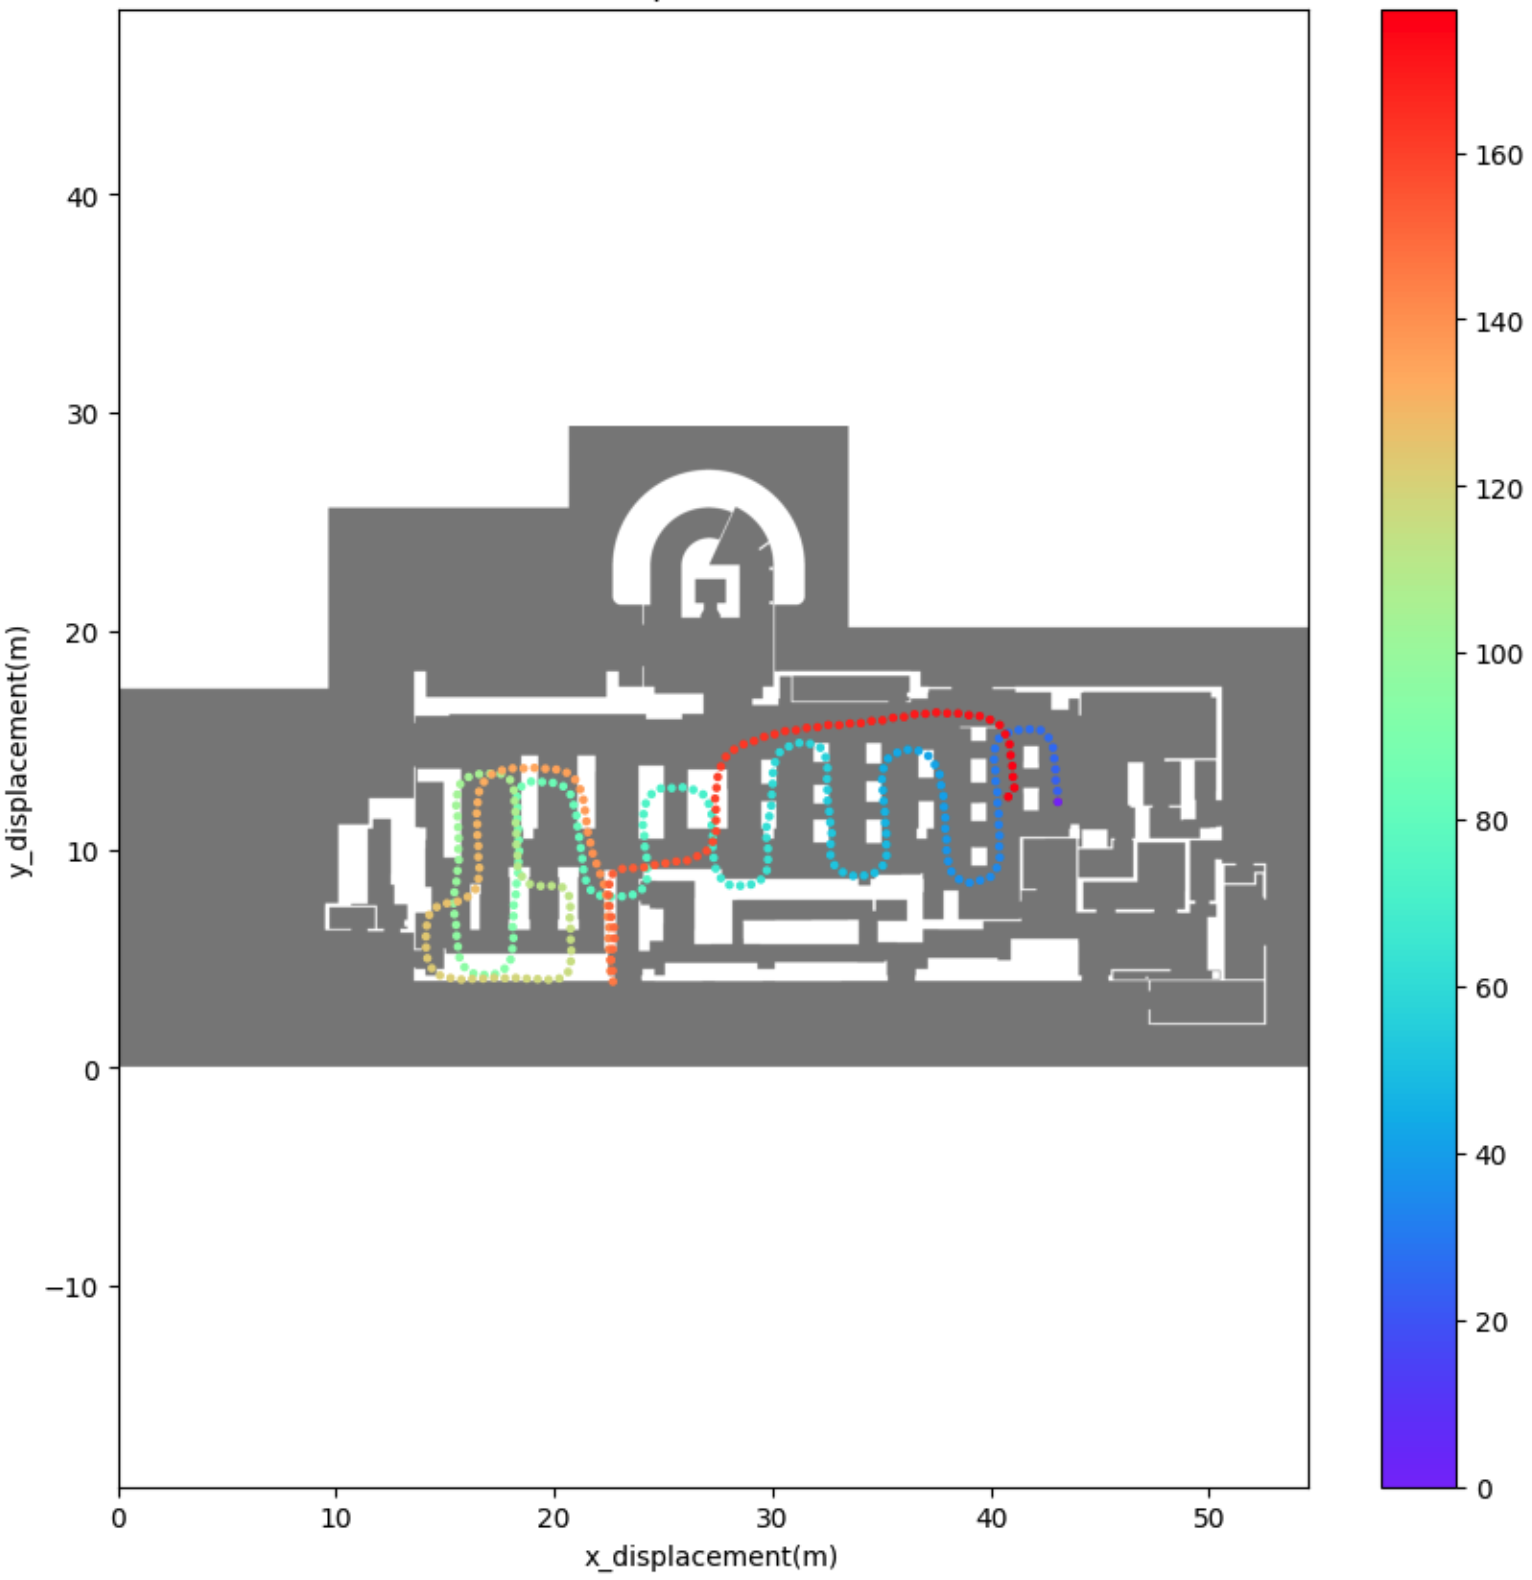
\includegraphics[width=\linewidth]{image/fingerprint-rotate.jpg}
	\caption{BLEのFPを補正後の軌跡}    \label{fig:fingerprint-rotate}
\end{figure}

\begin{lstlisting}[caption={BLEビーコンのFPを使用した\\初期進行方向補正}, label=lst:rotate-trajectory-using-ble-fingerprint,float =h]
def rotate_trajectory_to_optimal
          _alignment_using_ble_fingerprint(
    acc_df: pd.DataFrame,
    angle_df: pd.DataFrame,
    ble_scans_df: pd.DataFrame,
    ble_fingerprint_df: pd.DataFrame,
    floor_name: str,
    ground_truth_first_point: dict[Axis2D, float]
) -> tuple[pd.DataFrame, pd.DataFrame]:                                        
\end{lstlisting}



\subsection{フロアマップを用いた歩行可能領域への補正}

図\ref{fig:pdr-rotate}に示す軌跡の問題点として人間が歩行不可能領域を通過している点がある.
現実の人間がこのような場所を通過しないため,このような軌跡は不適切である.
そのため軌跡が歩行不可領域に存在する場合は,歩行可能な領域に移動させる処理が必要である.
この問題を解決する処理としてListing\ref{lst:map-matching}にマップマッチング補正関数を示す.
マップマッチング補正関数は引数に加速度DF,角度DF,フロアマップ情報DICT,フロア名,マップの1pxあたりの距離を取る.
戻り値は座標DFのみを返す.内部の処理の関係上,補正後の角度DFは返すのが難しいためである.
関数内部ではまず加速度と角度のデータを基にして軌跡を推定する.
この軌跡に対して,各地点での座標が与えられたフロアマップ上の歩行可能な領域に存在するかどうかを検証する.
検証の結果,各地点での座標が歩行不可能な領域に存在する場合,当該座標から最も近い歩行可能な座標を幅優先探索アルゴリズムを
用いて探す.
該当する座標が見つかった場合,該当座標と該当座標以降の軌跡の座標を歩行可能な座標に平行移動して補正を行う.
当該座標の補正が終了後,次の座標に対して同様の処理を行う処理を繰り返す.
これによって軌跡の各地点が歩行可能な領域に存在するようになり,軌跡全体が最適化される.
図\ref{fig:map-matching}に示すように,マップマッチング補正後の軌跡では
歩行不可能な領域に存在していた地点が歩行可能な地点に移動されている.

\begin{lstlisting}[caption={マップマッチング補正}, label=lst:map-matching]
def move_unwalkable_points_to_walkable(
    acc_df: pd.DataFrame,
    angle_df: pd.DataFrame,
    map_dict: dict[str, np.ndarray],
    floor_name: str,
    dx: float,
    dy: float,
    ground_truth_first_point: dict[Axis2D, float]
) -> pd.DataFrame:

\end{lstlisting}

\begin{figure}[h]
	\centering
	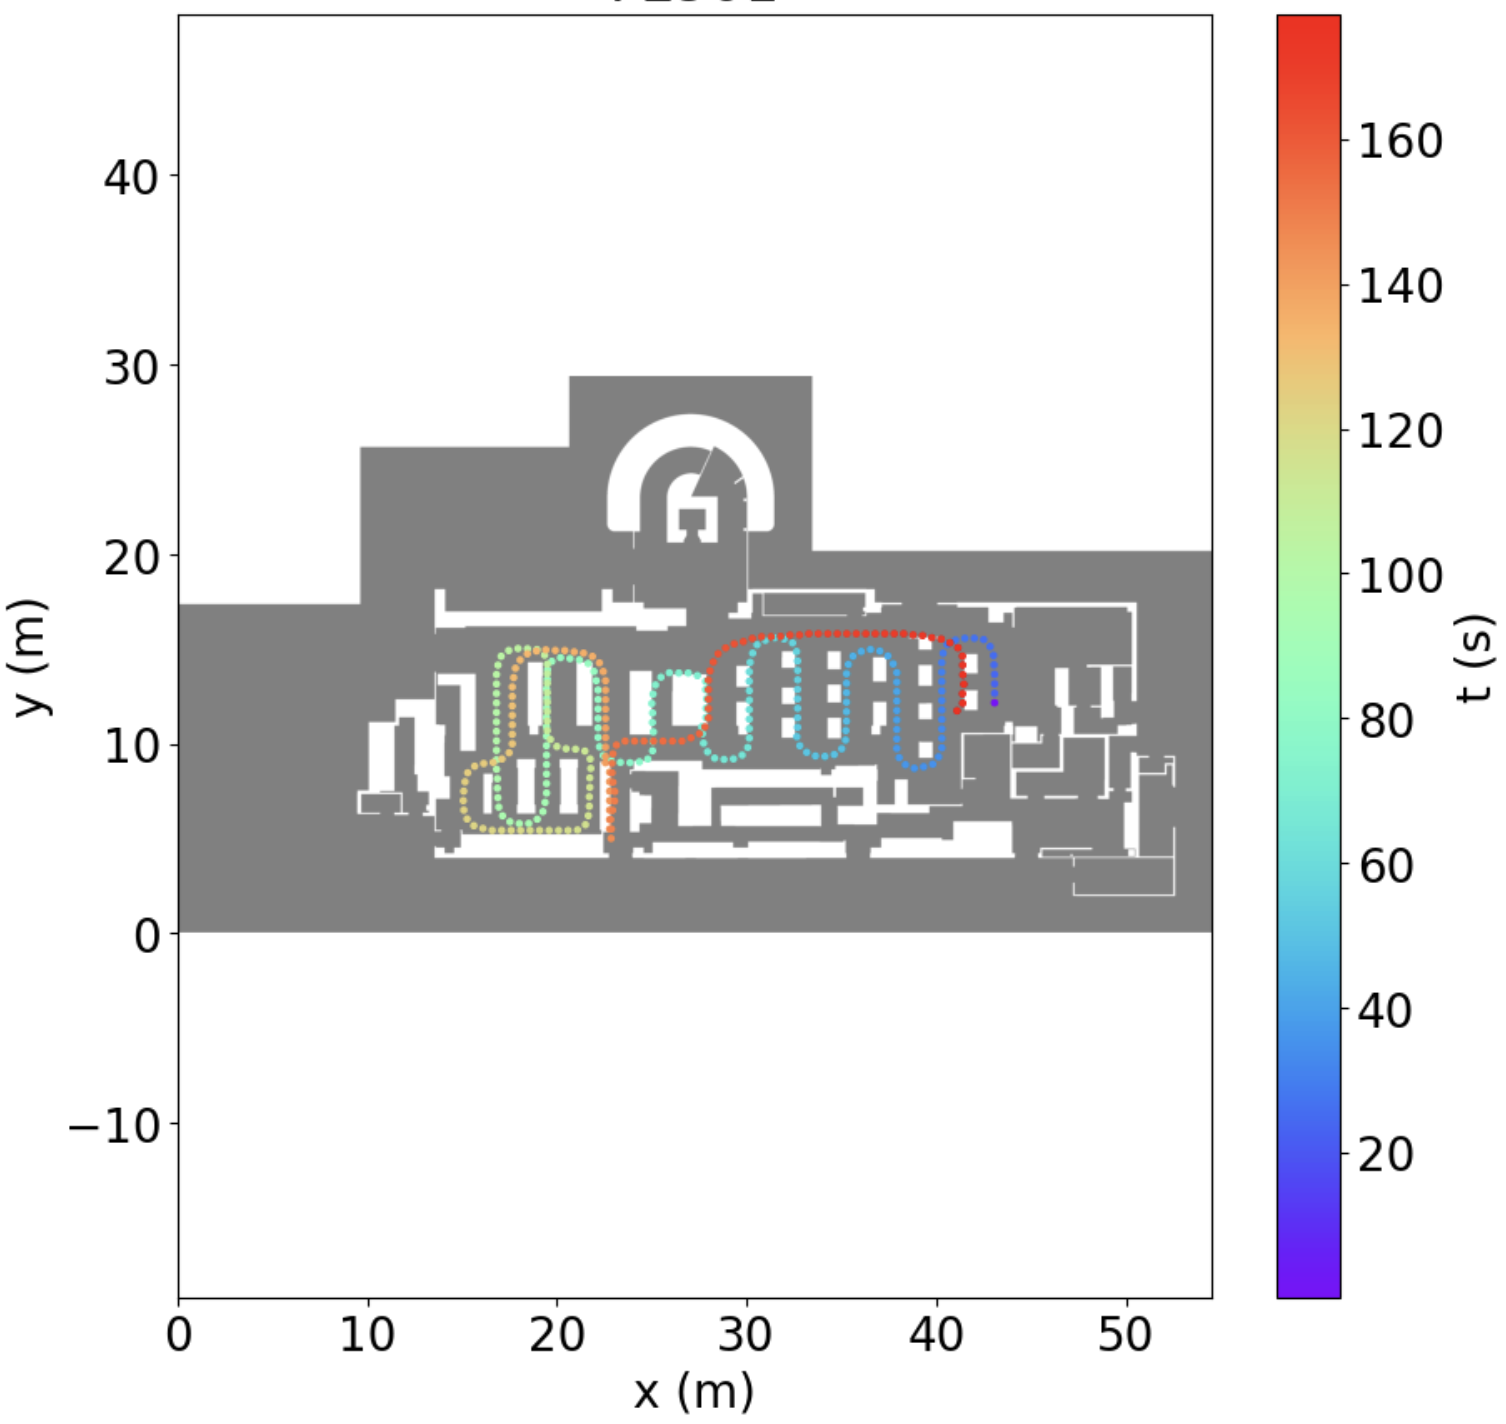
\includegraphics[width=\linewidth]{image/map-matching.jpg}
	\caption{マップマッチング補正後の軌跡}    \label{fig:map-matching}
\end{figure}




\subsection{気圧データを用いた3次元的な位置推定}



